\section{Apache S4}


Nach der Vorstellung von Apache Storm, Kafka und Flume wird in diesem Kapitel Apache S4 vorgestellt. Apache S4 ist eine Abkürzung und steht für Simple Scalable Streaming System und wird von Flavio Junqueira als allgemeine, verteilte, skalierbare, teilweise fehlertolerante, steckbare Plattform bezeichnet \citeint{s4:Proposal}. Zunächst soll eine Kurzübersicht einen ersten Einblick in Apache S4 geben. Anschließend werden die Bewertungskriterien erläutert und vorgestellt.

\begin{table}[tbp]
	\centering
		\begin{tabular}{@{}ll@{}} \toprule
			\textbf{Faktum} & \textbf{Beschreibung} \\ \midrule
			Hauptentwickler & Matthieu Morel, Kishore Gopalakrishna, Flavio Junqueira \\
			& Leo Neumeyer, Bruce Robbins, Daniel Gomez Ferro \\
			Stabile Version & 0.6.0 vom 03.06.2013 \\ 
			Entwicklungsstatus &  Moderat \\
			Entwicklungsversion & 0.7.0 \\
			Sprache & Java \\
			Betriebssystem & plattformunabhängig, benötigt die Java Virtual Machine \\
			& und Apache Zookeeper \\
			Lizenz & Apache License version 2.0 \\
			Webseite & \citeint{s4:home} \\
			Quelltext & \citeint{s4:GitHubApacheMirror} \\			
			\bottomrule			
		\end{tabular}
	\caption{Kurzübersicht Apache S4}
	\label{tab:vors4}
\end{table}


Die Architektur von Apache S4 baut auf einem Apache Zookeeper Cluster auf und besteht aus mehreren Apache S4 Cluster, Nodes, Apps und Processing Elements. Apps sind Java Archive die in einem Apache S4 Cluster bereitgestellt werden. Die Größe eines Clusters entspricht der Anzahl der Tasks. Pro Task muss jeweils eine Apache S4 Node als selbständiger Prozess gestartet werden. Apps bestehen aus einem Graph aus Processing Elements und Streams. Ein Processing Element kommuniziert über unterschiedliche Clustern per Streams miteinander asynchron. Eine Nachricht erbt von der Klasse Event, besteht aus einem Schlüssel/Wert-Tupel und wird in einem Stream verpackt und versendet. Mit der Erweiterung der Basisklasse AdapterApp kann ein Stream erzeugt werden. Ein Beispiel wird im Anhang \ref{lst:s4HelloInputAdapter} gezeigt. Dabei wird auf eine Netzwerkverbindung mit dem Anschluss 15000 gehört. Bei erfolgreicher Verbindung wird der Inhalt gelesen und in den Stream gesetzt. In einem Processing Element wird die Datenverarbeitung durchgeführt. Spezielle Aggregate und Operatoren von Nachrichten müssen daher in Processing Elements-Klassen implementiert werden. Ein Processing Element besteht aus Zwei Teilen, dem Prototype und der Instance. Der Prototype erbt von der Basisklasse ProcessingElement und behandelt eingehende Nachrichten. Die Instance erbt von der Basisklass App und behandelt den Anwendungsstart und -stop. Im Anhang \ref{lst:s4HelloAppProcessingElementInstance} wird ein Beispiel für das Erzeugen eines Streams "`names"' und die Weitergabe der Nachrichten gezeigt. \citeint{s4:overview}

In Abbildung \ref{fig:s4HelloApp} wird das Beispiel \ref{s4:beispielHelloApp} aus der Apache S4 Installation im Anhang \ref{sec:s4install} gezeigt. Zuerst werden Zwei Cluster cluster1 und cluster2 in einem Apache Zookeeper Cluster bereitgestellt. Anschließend wird im Repository die S4 Anwendung myApp hinzugefügt. Die Apache Zookeeper nodes werden informiert und die Anwendung wird gestartet. Ein neuer Stream "`names"' wird erstellt und beide nodes werden als Consumer registriert. Anschließend wird im Cluster cluster2 die Adapter-Anwendung gestartet. Beim Bereitstellen der Anwendung im Cluster cluster2 wird der Stream "'names"' als Identität für den Ausgabestrom gesetzt. Die Adapter-Anwendung ist nach dem Starten aktiv und wartet auf Dateneingang. Abschließend werden eintreffende Daten vom Cluster cluster2 in S4 Nachrichten umgewandelt und zur weiteren Datenbehandlung an die Consumer verteilt.

\begin{figure}[htb!]
\centering
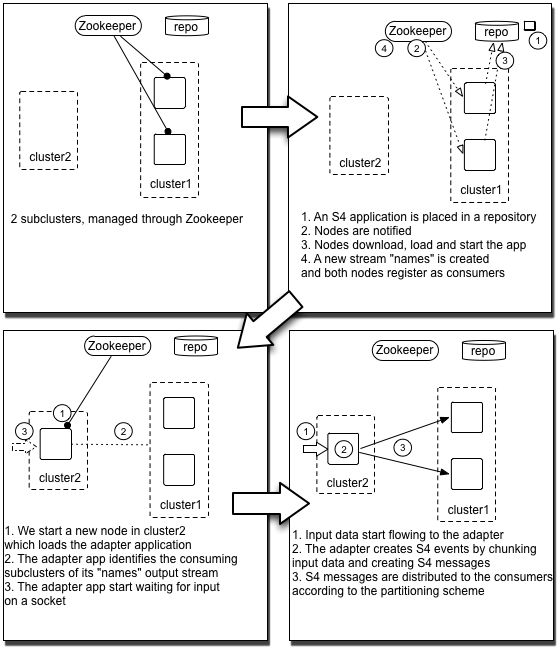
\includegraphics[width=1.0\textwidth]{bilder/s4SampleAppDeployment.png}
\caption{Apache S4 HelloApp Beispiel
\label{fig:s4HelloApp}}
\end{figure}

Nachrichten werden in Apache S4 zwischen den Nodes durch den Communication Layer übertragen. Der Communication Layer nutzt für die Koordination der Nachrichten zwischen den Apache S4 nodes Apache Zookeeper. Es werden Bindungen in verschiedenen Programmiersprachen angeboten, um Nachrichten an die Nodes im Apache S4 Cluster zu senden. Durch ein steckbares Design können unterschiedliche Nachrichtenprotokolle wie zum Beispiel Apache Avro oder Apache Thrift eingesetzt werden. Eine Implementierung für \gls{glo:udp} \citeint{s4:classUdpEmitter} und \gls{glo:tcp} \citeint{s4:classTcpEmitter} wird von Apache S4 bereits unterstützt. \citelit[S. 4, Kap. II D]{s4:Neumeyer}

Die Fehlertoleranz in Apache S4 wird durch die Fail-Fast Strategie von Apache Zookeeper übernommen. In einem Apache S4 Cluster mit Zwei Tasks und Vier gestarteten Nodes, sind Zwei Nodes Aktiv und Zwei Nodes im Standby-Betrieb. Wenn Apache Zookeeper einen Session-Timeout einer aktiven Node feststellt, wird sofort eine Standby-Node aktiviert, die anderen Nodes werden über die neue aktive Node informiert und neue Nachrichten werden umgeleitet. Apache S4 Nodes speichern nutzen für die Datenverarbeitung den lokalen Speicher von Apache Zookeeper. Im Fehlerfall geht der Zwischenspeicher einer Apache Zookeeper Node verloren. Damit die Daten nicht verloren gehen, kann mit dem Checkpointing Mechanismus über die Konfiguration eine Datensicherung in einem externen Datenlager erfolgen. \citeint{s4:faultTolerance}

\begin{table}[ht!]
	\centering
		\begin{tabular}{@{}ll@{}} \toprule
			\textbf{Kriterium} & \textbf{Bewertung} \\ \midrule
			Architektur & Strukturierte Peer-to-Peer-Architektur \\
			Prozesse und Threads & Client-Server-Modell \\
			Kommunikation & TCP-basiert und UDP-basiert via Apache Zookeeper \\
			Namenssystem & Hierarchische Benennung \\
			Synchronisierung & Processing Elements werden synchronisiert\\
			Pipelining und Materialisierung & Chaining von Processing Elements  \\
			Konsistenz und Replikation & Consistent hashing, Checkpointing \\
			Fehlertoleranz & Load balancing und Failover \\ 
			Sicherheit & Nur eigene Maßnahmen \\
			& Monitoring mit JMX pro Node \\
			Erweiterung & Modulare Eigenentwicklung und Community-Beiträge \\
			Qualität & \gls{glo:ttl} \\
			\bottomrule			
		\end{tabular}
	\caption{Bewertung Apache S4}
	\label{tab:bews4}
\end{table}
